\chapter{Esperiments}

\label{ch:experiments}

In this Chapter, we'll use the \texttt{atarieyes} software to test the
effectiveness of the ideas presented in this thesis. The purpose of these
experiments is both to demonstrate that a features extractor can be learnt
with the method proposed, and to show how these features can be used
in combination with the Restraining Bolt for complex RL tasks.

We'll look at two environments: Breakout and Montezuma's Revenge. For the
first we'll test the training process of the features extractor, while the
second is used for a more complete demonstration about the possibilities (we
proceed from learnt features to the application of the Restraining Bolt).

% Page too short: don't break here
\let\sectionbreak\dontbreakhere

\section{Breakout}

\label{sec:exp-breakout}

The first environment we'll see is the famous Atari game ``Breakout''.
A frame of this game is shown in Figure~\ref{fig:breakout-frame}.
\begin{figure}
	\centering
	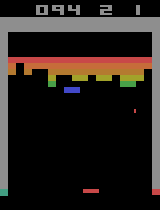
\includegraphics[height=3cm]{./imgs/br1.png}
	\caption{A frame from the Atari game ``Breakout''.}
	\label{fig:breakout-frame}
\end{figure}
The goal is to hit all the bricks with the ball (the small orange dot). Every
time one brick is eliminated, the environment produces a positive reward. The
agent, through the four actions available, \const{NoOp}, \const{Fire},
\const{Right} and \const{Left}, can move the paddle at the bottom and direct
the ball. Every time the paddle misses the ball, the agent loses a life.
However, during training, we terminate and reset the episode at this event.

The exact environment name for this game is \verb|BreakoutDeterministic-v4|.


\subsection{Definitions}

We now define two propositional symbols, \const{Full} and \const{Empty}, and
we apply the proposed model and training procedure to learn their Boolean
valuation function. The intended interpretation of these two proposition
is:
\begin{description}
	\item [\const{Full}] should be true when the area is full of bricks.
	\item [\const{Empty}] should be true when there are no bricks inside the
		area.
\end{description}
The area which we're talking about is shown in
Figure~\ref{fig:breakout-fluents}. The orange rectangle which contains the
intended set of bricks is also the fluents region. So, we've defined two
symbols in one region of the image.
\begin{figure}
	\centering
	\begin{tikzpicture}
		\node [image, tight] (env-br)
			{
\includegraphics[height=4cm]{./imgs/br2.png}};
		\begin{scope}[shift=(env-br.north west), x={(env-br.north east)},
			y={(env-br.south west)}]
			\draw [region box] \boxblueright node (blueright-coord) {};
		\end{scope}
		\matrix (br-fluents) [right=of env-br,
				matrix of nodes, nodes={anchor=west}] {
			\texttt{full}: true when shot 0 of 18 bricks down \\
			\texttt{empty}: true when shot 18 of 18 bricks down \\
		};
		\draw [->, gray] (br-fluents-1-1.west) to (blueright-coord);
		\draw [->, gray] (br-fluents-2-1.west) to (blueright-coord);
	\end{tikzpicture}
	\caption{In this environment we define two fluents and one region.}
	\label{fig:breakout-fluents}
\end{figure}

How could we \emph{describe the behaviour} of these two propositions with
temporal logic? When an episode starts, we know that \const{Full} should be
true, because all bricks are present, initially. This initial condition is
really helpful. Then, \const{Full} and \const{Empty} represent concepts that
are always mutually exclusive. Finally, since the bricks cannot reappear, we
know that the path is forced: the propositions can't return to a previous
configuration. All these descriptions translate to the following \ldl{}
temporal constraint:
\begin{equation}
	\begin{array}{ll}
		\const{Full}\, \land &
		\to \text{initial condition}\\
		\lbox{\true^*} (\lnot \const{Full} \lor \lnot \const{Empty})\, \land &
		\to \text{exclusive propositions}\\
		\lnot \ldiamond{\true^*; \lnot \const{Full}; \true^*}
		(\const{Full} \land \lnot \lend)\, \land &
		\to \text{can't reappear}\\
		\lnot \ldiamond{\true^*; \const{Empty}; \true^*}
		(\lnot \const{Empty} \land \lnot \lend)\, \land \\
		\lnot \ldiamond{\true^*; \const{Full}} \const{Empty} &
		\to \text{not immediately}\\
	\end{array}
	\label{eq:breakout-constraint}
\end{equation}
The conjunction $\land \lnot \lend$ means that we're not referring to the end
of the trace. This is only required in this \ldl{} semantics for finite
traces.

The DFA associated to this temporal constraint is shown in
Figure~\ref{fig:breakout-constraint}. This is the automaton that the software
will use to search among the candidate functions.
\begin{figure}
	\centering
	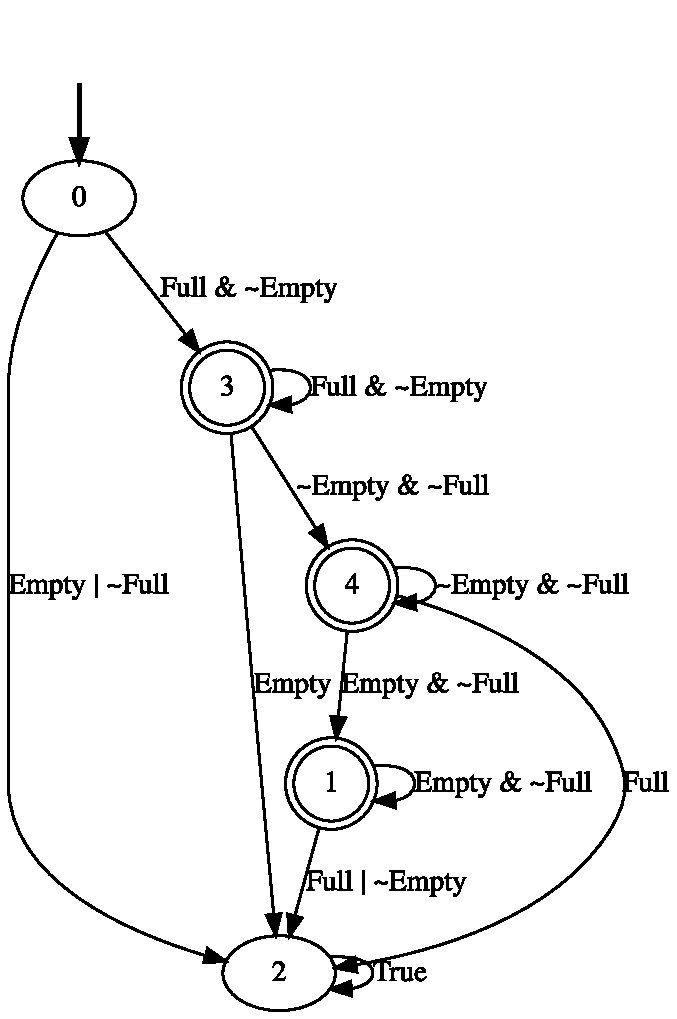
\includegraphics[height=0.5\textheight]{./imgs/br_constraints.pdf}
	\caption{The DFA associated to Equation~\eqref{eq:breakout-constraint}.}
	\label{fig:breakout-constraint}
\end{figure}
As we can see from its structure, the fluents dynamics is relatively simple.
We could have also used the following equivalent formula:
\begin{equation}
	\begin{aligned}
		&\ldiamond{(\const{Full} \land \lnot \const{Empty})^+}
			(\const{End} \,\lor \\
		&\qquad\ldiamond{(\lnot \const{Full} \land \lnot \const{Empty})^+}
			(\const{End} \,\lor \\
		&\qquad\qquad \ldiamond{(\lnot \const{Full} \land \const{Empty})^+}
			\const{End}))
	\end{aligned}
\end{equation}
where the operator $\resym^+$ is an abbreviation of the regular expression
$(\resym; \resym^*)$.
% TODO: draw with tikz

Most states in this automaton are final. In fact, nothing guarantees that the
agent will be able to hit the bricks in every episode. The fluents might not
evolve at all when the agent loses a play.

To specify all these definitions to our software we run:
\begin{lstlisting}[style=bash]
atarieyes features select -e BreakoutDeterministic-v4
\end{lstlisting}
and we select the region of Figure~\ref{fig:breakout-fluents}. Then we
complete the generated file with the fluents names and any of the two temporal
constraints above. The resulting file is shown in
Listing~\ref{lst:breakout-definitions}. 
\begin{listing}
	\begin{minted}{json}
{
  "_frame": [
    8, 32, 152, 197
  ],
	"regions": {
		"blue_right": {
			"abbrev": "br",
			"fluents": [
				"br_full",
				"br_empty"
			],
			"region": [
				32, 87, 152, 93
			]
		}
	},
	"constraints": [
		"br_full",
		"[true*](!br_full | !br_empty)",
		"!<true*; !br_full; true*>(br_full & !end)",
		"!<true*; br_empty; true*>(!br_empty & !end)",
		"!<true*; br_full>br_empty"
	]
}
	\end{minted}
	\caption{The content of \texttt{definitions/BreakoutDeterministic-v4.json}.}
	\label{lst:breakout-definitions}
\end{listing}
"\texttt{br}" is just an abbreviation for that region name. Other than that,
the file exactly represents what we've defined so far.


\subsection{Training}
\subsection{Comments}

% TODO: DQN con uno strato non bastava
% TODO: sembrava banale ma non lo è: natura combinatoria

% Back to brak into sections
\let\sectionbreak\savedsectionbreak

\section{Montezuma's Revenge}
\subsection{Definitions}
\subsection{Training}
\subsection{Comments}

% TODO: crossover and mutation p
